\documentclass[11pt,professionalfonts,aspectratio=169,final]{beamer}

\usepackage{research_summary_packages}
%\bibliography{library} % must be in the preamble when using biblatex package

\DeclareSIUnit\year{yr} % 2016AAS
\newcommand{\vs}{\vspace{0.3cm}} % 2016ACC

\definecolor{mygray}{gray}{0.9}
\definecolor{RoyalBlue}{rgb}{0.25,0.41,0.88}
\def\Emph{\textcolor{RoyalBlue}}

\definecolor{tmp}{rgb}{0.804,0.941,1.0}
\setbeamercolor{numerical}{fg=black,bg=tmp}
\setbeamercolor{exact}{fg=black,bg=red}

\mode<presentation> 
{
  \usetheme{Warsaw}
  \usefonttheme{serif}
  \setbeamercovered{transparent}
}

\setbeamertemplate{footline}%{split theme}
{%
  \leavevmode%
  \hbox{\begin{beamercolorbox}[wd=.5\paperwidth,ht=2.5ex,dp=1.125ex,leftskip=.3cm,rightskip=.3cm plus1fill]{author in head/foot}%
    \usebeamerfont{author in head/foot}\insertshorttitle
  \end{beamercolorbox}%
  \begin{beamercolorbox}[wd=.5\paperwidth,ht=2.5ex,dp=1.125ex,leftskip=.3cm,rightskip=.3cm]{title in head/foot}
%    \usebeamerfont{title in head/foot}\mypaper\hfill \insertframenumber/\inserttotalframenumber
    \usebeamerfont{title in head/foot}\hfill \insertframenumber/\inserttotalframenumber
  \end{beamercolorbox}}%
  \vskip0pt%
} \setbeamercolor{box}{fg=black,bg=yellow}


\title[Research Summary]{\large\bf  Professor Chrikjian Visit}

\author{Shankar Kulumani}

%\institute{\footnotesize
%{\normalsize Shankar Kulumani}\vspace*{0.2cm}\\
%  Flight Dynamics and Control Lab \\ 
%  Dept. of Mechanical and Aerospace Engineering\\ 
%  The George Washington University \\
%  Washington, DC\\ \vspace{10pt}
%  June 4, 2014 \\ \vspace{10pt}
%  }
\date{29 September 2016}

\institute{
\large{\textbf{Flight Dynamics \& Control Lab}}\\
  \begin{figure} %figure%
        
\includegraphics[width=0.75\textwidth]{gw_txh_2cs_pos}
    \end{figure}
}


\begin{document}
%=======================================================%

\setcounter{framenumber}{-1}
\begin{frame} %-----------------------------%
  \titlepage
\end{frame}   %-----------------------------%

\section{Orbital transfers using Reachability}
\subsection{Motivation}

\begin{frame} %-----------------------------%
\frametitle{Low-thrust vehicles} % electric propulsion
\begin{itemize}
    \item Low-thrust orbital transfers offer increased mission oportunities
    \begin{itemize}
        \item Electric propulsion is increasing in capability
        \item Offers much higher specific impulse than chemical engines 
        \item Requires much longer operating periods for maneuvers 
        \item Enables long duration missions with frequent thrusting
    \end{itemize}
\end{itemize}

\begin{center}
    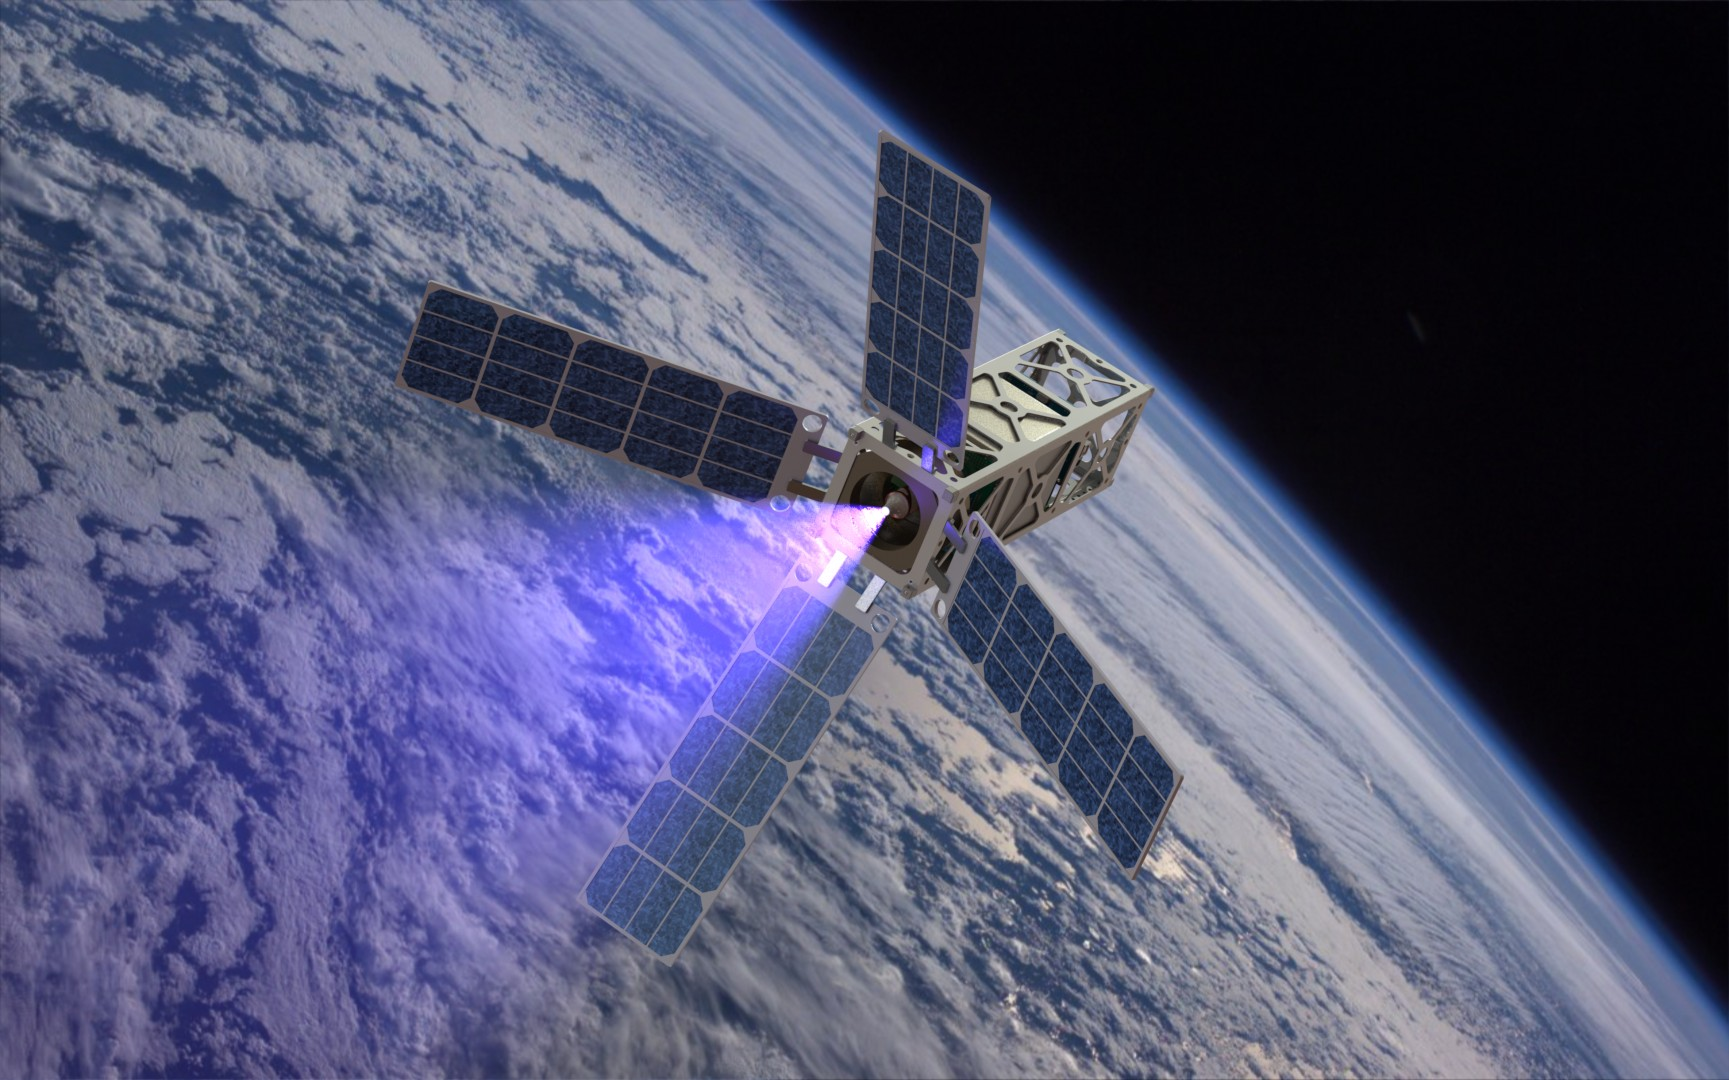
\includegraphics[height=0.3\textheight]{figures/patriot_plume.jpg}
    ~
    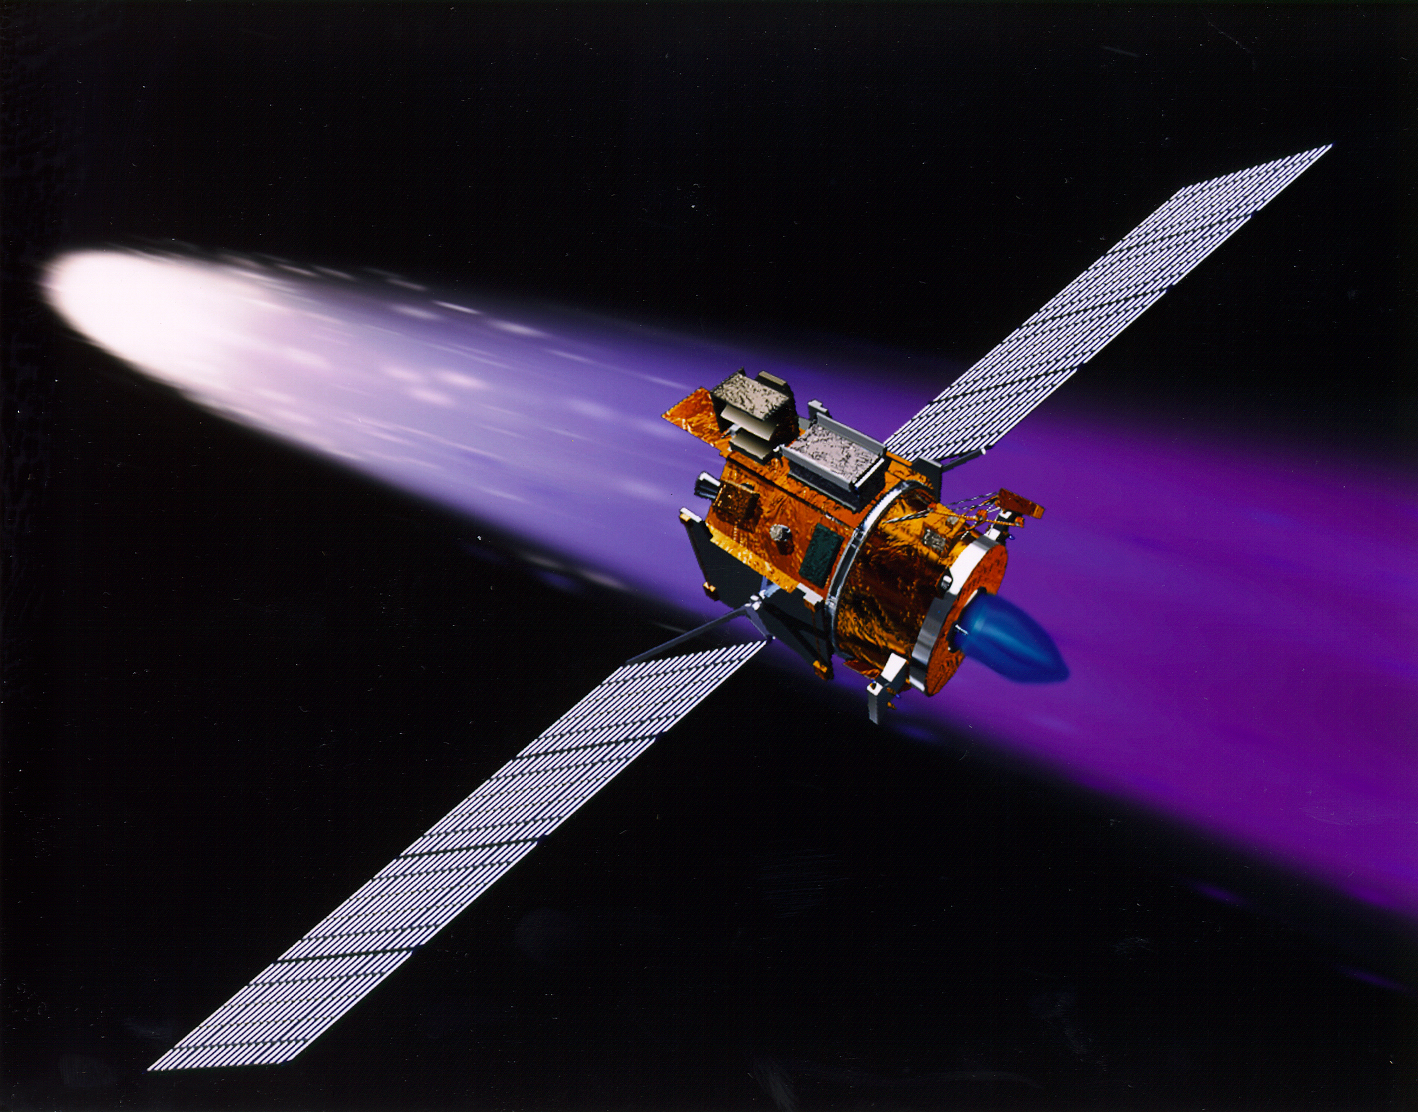
\includegraphics[height=0.3\textheight]{figures/deepspace1.jpg}
\end{center}
\end{frame}   %-----------------------------%

\begin{frame}{Asteroid Missions}
\begin{itemize}
    \item Science - insight into the early formation of the solar system
    \item Mining - vast quantities of useful materials
    \item Impact - high risk from hazardous near-Earth asteroids
\end{itemize}    

\begin{center}
    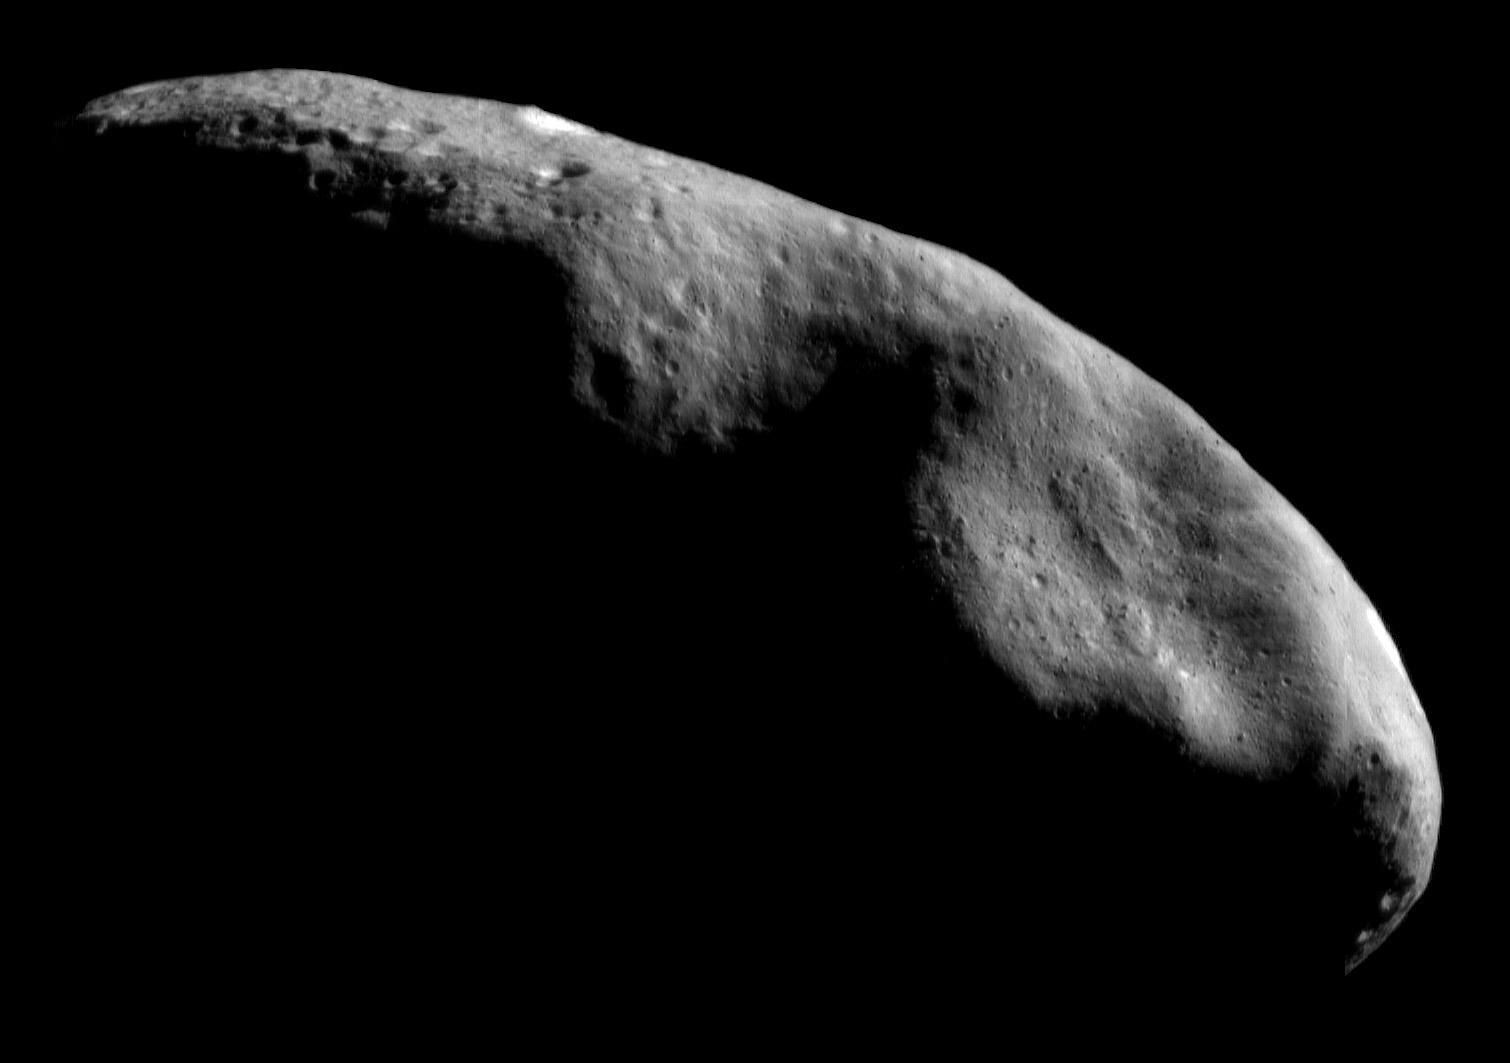
\includegraphics[height=0.35\textheight]{figures/2016AAS/near_mos_20001203_full.jpg}
    \hfill
    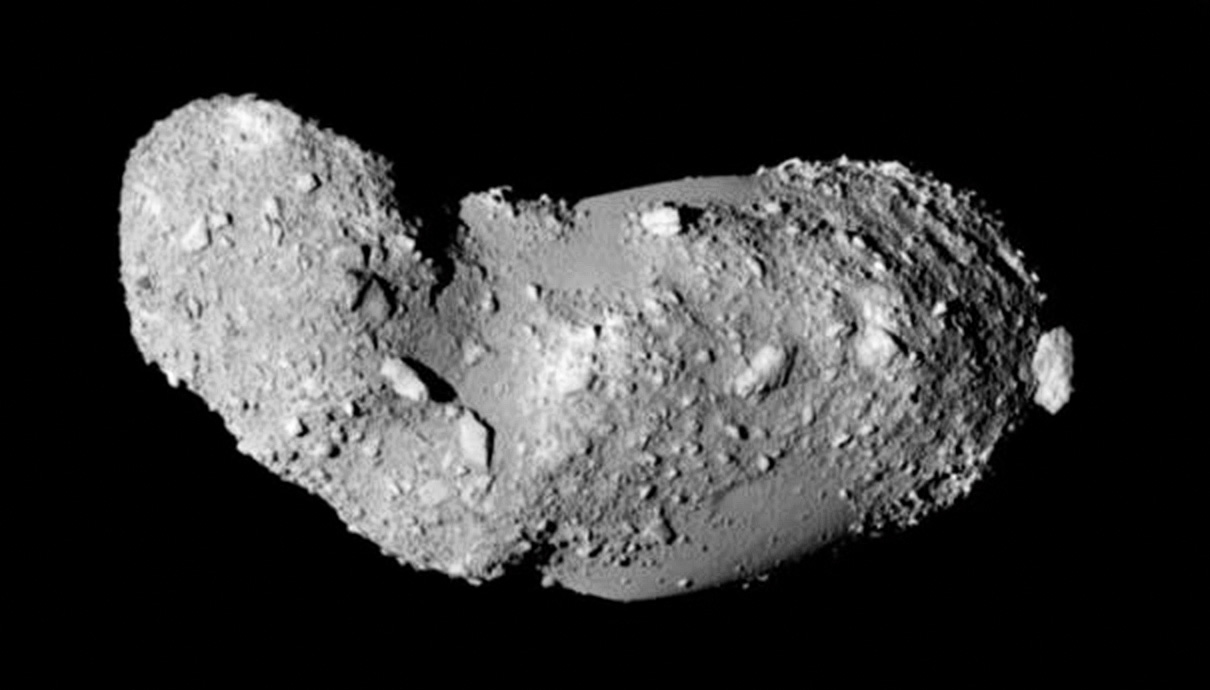
\includegraphics[height=0.35\textheight]{figures/2016AAS/Itokawa8_hayabusa_1210.jpg}
\end{center}
\end{frame}

\begin{frame}{Asteroid Mining}
    \begin{itemize}
      \item Useful materials can be extracted from asteroids to support:
      \begin{itemize}
          \item Propulsion, construction, life support, agriculture, and precious/strategic metals
      \end{itemize}
      \item Commercialization of near-Earth asteroids is feasible~\footfullcite{ross2001}
    \end{itemize}

\pause

\begin{center}
\small
    \begin{tabular}{|l|r|r|}
        \hline 
        Element & Price (\SI{}{\$\per\kilo\gram}) & Sales (\SI{}{\$M\per\year}) \\
        \hline \hline 
        Phosphorous (P) & \num{0.08}  & \num{2167} \\
        Gallium (Ga) & \num{300.00}  & \num{1544} \\
        Germanium (Ge) & \num{745.00} & \num{6145} \\
        \hline \hline 
        Platinum (Pt) & \num{12394.00} & \num{1705} \\
        Gold (Au) & \num{12346.00} & \num{49} \\
        Osmium (Os) & \num{12860.00} & \num{307} \\
        \hline
    \end{tabular}
\end{center}

\end{frame}



\begin{frame}{Challenges for Optimal Transfer Design} %-----------------------------%

\begin{itemize}
    \item Optimal Trajectory Design
        \begin{itemize}
            \item Orbital dynamics are nonlinear and chaotic
            \item Very sensitive to initial conditions
            \item Intuition required by designer to enable convergence
        \end{itemize}
    \pause
    \item Transfers using low-thrust propulsion
        \begin{itemize}
            \item Requires long periods of thrusting/coasting
            \item Small perturbations require accurate numerical integration
            \item Difficult to capture the long-term effects accurately
        \end{itemize}
    \pause
    \item Direct Optimal Control
        \begin{itemize}
            \item Reformulate problem as parameter optimization
            \item Allows for use of nonlinear programming methods
            \item High dimensional problem and computationally intensive
            \item Results in suboptimal solutions due to discretization
        \end{itemize}
\end{itemize}
\end{frame}   %-----------------------------%

\subsection{Approach}

\begin{frame}{Proposed Approach} % -----------------------------------%
  \begin{itemize}
      \item \Emph{Reachability set} on \Poincare section allows for systematic transfer design
        \begin{itemize}
            \item Transfer design on lower dimensional subspace
            \item Simple method to incorporate effects of low-thrust 
            \item Avoids the issue of determining initial conditions
        \end{itemize}
        \pause
      \item Extension of previous work in planar three-body problem     
  \end{itemize}

  \note[itemize]{
    \item Reachability set avoids the need to pick initial conditions
    \item We compute on a lower dimensional surface
  }
\end{frame} %--------------------------------------%

\begin{frame}{\Poincare map}
\begin{itemize}
    \item Intersection of a periodic orbit with a lower dimensional subspace, called the \Poincare section
    \pause
        \begin{itemize}
            \item Can be considered a discrete map 
        \end{itemize}
        \pause
    \item Useful for investigating the stability and structure 
    \pause
    \item Define a \Poincare section \( \Sigma \) 
        \begin{itemize}
            \item Used for initial and target periodic orbits
            \item Subspace for the \Emph{reachability set}
        \end{itemize}
\end{itemize}

\begin{align*}
    \Sigma = \braces{\parenth{x, \dot{x}, z, \dot{z}} | y(t_f) = 0 }
\end{align*}

\end{frame}

\begin{frame}{Reachability Set}

\begin{itemize}
    \item Set of states achievable from a given initial condition over fixed \( t_f \) s.t. maximum control constraint
    \begin{align*}
        R( \vecbf{x}_0, \mathcal{U} , t_f) = \braces{ \vecbf{x}_f \subseteq \mathcal{X} | \exists \vecbf{u} \in \mathcal{U}, \vecbf{x}(t_f) = \vecbf{x}_f }
    \end{align*}
    \pause
    \item Directly derivable from optimal control
    \item Frequently used for safety planning, e.g. air traffic collision avoidance
    \pause
    \item We extend its use to the design of spacecraft transfers
\end{itemize}

\end{frame}

\begin{frame}{Reachability Set on \Poincare section} % -----------------------------------%

\begin{itemize}
    \item Generate the reachability set on a \Poincare section
    \[
        \Sigma = \braces{\parenth{x, \dot{x}, z, \dot{z}} | y(t_f) = 0 }
    \]
    \item Control input is chosen to enlarge the reachable set
\end{itemize}
\pause
\begin{figure}
    \centering
    \begin{scaletikzpicturetowidth}{0.4\textwidth}
    \begin{tikzpicture}[scale=\tikzscale]
        \coordinate [label=left:\textcolor{black}{\large \(\vecbf{x}_0\)}] (x0) at (-1,-2);
        \coordinate [label=below:\textcolor{black}{\large  \(\vecbf{x}_n\)}] (xn) at (1,1);
        \coordinate [label=left:\textcolor{black}{\large  \(\Sigma\)}] (sigma) at (-4,3);
        %\coordinate [label=below:\textcolor{black}{\large  \(P(\vec{x})\)}] (P) at (0,-3.5);
        % define the path of the flow with coordinates
        \coordinate [label=right:\textcolor{black}{}] (f1) at (5,-2);
        \coordinate [label=below:\textcolor{black}{\large  \(\psi(t,\vecbf{x}_0)\)}] (f2) at (2,-5);
        \coordinate [label=right:\textcolor{black}{}] (f3) at (-4,-4);
        \coordinate [label=right:\textcolor{black}{}] (f4) at (-4,-1);
        
    %   \draw[help lines] (-10,-10) grid (10,10); %grid
        \filldraw [black] (x0) circle [radius=3pt];
        \filldraw [black] (xn) circle [radius=3pt];
    
        \draw [ultra thick,black,->-](x0) to[out=20,in=90,distance=2cm] (f1) to[out=-90,in=0,distance=2cm] (f2) to[out=180,in=-45,distance=2cm] (f3) to[out=135,in=-135,distance=2cm] (f4) ;
        \draw [ultra thick, black,dashed,->] (f4) to[out=45,in=180,distance=1cm] ($(xn)-(2,0)$);
        
        \draw [ultra thick] plot [smooth cycle, tension=0.1, rotate=5] coordinates { (-4,-3) (4,-3) (4,3) (-4,3) };
    
        \draw [thick,dashed] (xn) circle [radius=2cm]; % reachability set
    
        \draw [thick,->] (xn) -- ($(xn) + (2.5,0)$);
        \draw [thick,rotate=45,->] (xn) -- ($(xn) + (2.5,0)$);
        \draw ($(xn) + (1,0)$) arc [start angle=0,end angle=45, radius=1];
        \node [draw=none] at (2.8,1.5) {\large \(\phi_d\)};
        \draw [decorate,decoration={brace,amplitude=5pt},rotate=45] (xn) -- ($(xn) + (2,0)$);
        \node [draw=none] at ($ (xn) + (0,1) $) {\large \( J \)};
    \end{tikzpicture}
    \end{scaletikzpicturetowidth}
\end{figure}

\end{frame} %--------------------------------------%

\begin{frame}{Optimal Control Problem}
\begin{itemize}
    \item Reachability defined as distance between controlled and uncontrolled states
    {\small
        \[
            J = -\frac{1}{2} \left( \vecbf{x}(t_f) - \vecbf{x}_{n}(t_f)\right)^T 
            Q
            \left( \vecbf{x}(t_f) - \vecbf{x}_{n}(t_f)\right) 
        \]
    }
    \pause
    \item Terminal constraints used to ensure correct section and specific direction on \( \Sigma \in \R^4 \)
    {\small
        \begin{align*}\label{eq:terminal_constraints}
            \begin{split}
                m_1 &= y = 0  \\
                m_2 &= \parenth{\sin \phi_{1_{d}}} \parenth{ x_1^2 + x_2^2 + x_3^2 + x_4^2} - x_1^2 = 0 \\
                m_3 &= \parenth{\sin \phi_{2_{d}}} \parenth{ x_2^2 + x_3^2 + x_4^2} - x_2^2 = 0\\
                m_4 &= \parenth{\sin \phi_{3_{d}}} \parenth{ 2 x_3^2 + 2 x_3 \sqrt{x_4^2 + 2 x_4^2}} - x_3 - \sqrt{x_4^2 + x_3^2} = 0 
            \end{split}
        \end{align*}
    }
    \pause
    \item Control constraint used to emulate realistic system
        {\small
        \[
            c(\vecbf{u}) = \vecbf{u}^T \vecbf{u} - u_m^2 \leq 0 
        \]
        }
\end{itemize}

\end{frame}

\begin{frame}{Two Point Boundary Value Problem}
\begin{itemize}
    \item Multiple shooting used to solve necessary conditions
    \pause
    \item Approximate the reachable set via \( \phi_1, \phi_2, \phi_3 \) 
    \pause
    \item From the reachable set we chose the state which minimizes \( d \) 
    \item Compute another reachable set if target is not feasible
\end{itemize}

\begin{align*}
    d = \sqrt{k_x \parenth{x_f - x_t }^2 + k_z \parenth{z_f - z_t }^2 + k_{\dot{x}}\parenth{\dot{x}_f - \dot{x}_t }^2 + k_{\dot{z}}\parenth{\dot{z}_f - \dot{z}_t }^2} 
\end{align*}

\end{frame}

\begin{frame}{Numerical Simulation}
\begin{itemize}
    \item Reachability approach applied to two dynamical systems
    \begin{itemize}
        \item Planar Circular Restricted Three Body Problem
        \item Two-body motion about asteroids
    \end{itemize}
    \item Extension from planar to 3D motion 
    \item Inclusion of complex gravitional field
\end{itemize}

\end{frame}

\subsection{CRTBP Simulation}

\begin{frame}{Geostationary to \( L_1 \) transfer} %----------------------------------------------------%
\begin{itemize}
       \item Tranfer for geostationary orbit to a periodic orbit about \( L_1\)
       \item Multiple iterations of reachable set
\end{itemize}

\begin{figure}
       \centering
       \begin{subfigure}[htbp]{0.5\textwidth}
               \only<1>{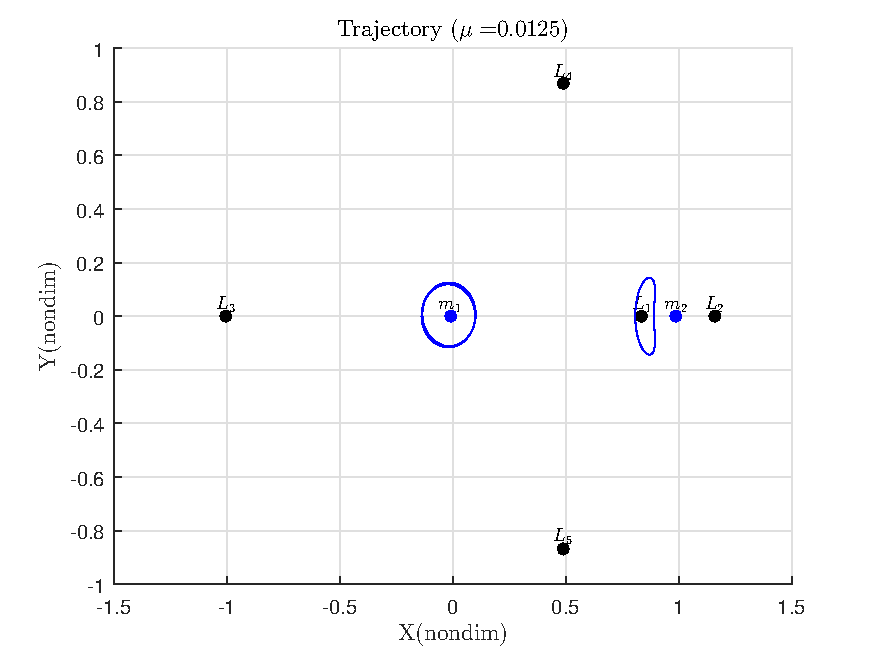
\includegraphics[width=\textwidth]{initial_final}  }
               \only<2>{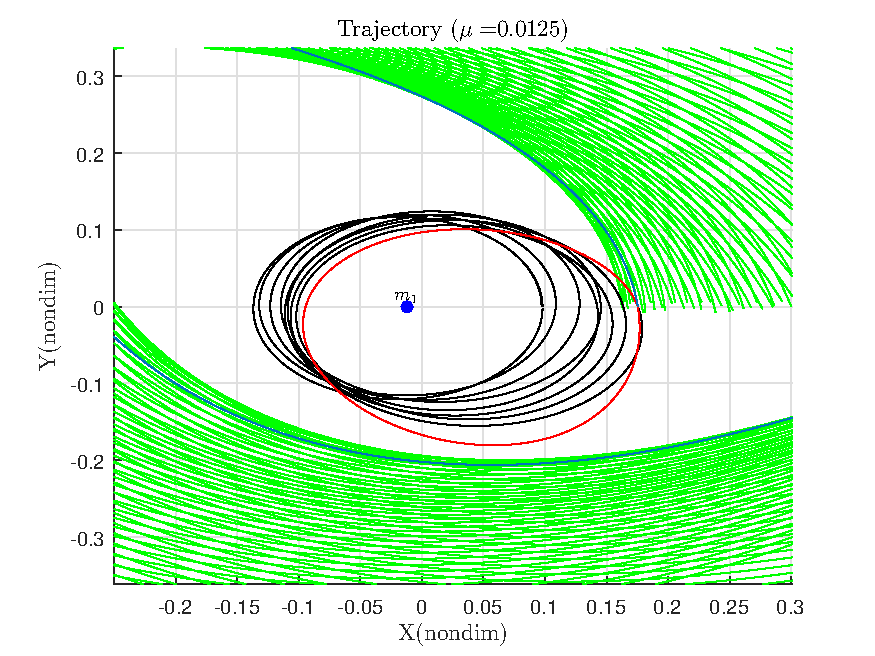
\includegraphics[width=\textwidth]{geo_transfer_zoom}  }
       \end{subfigure}~
       \begin{subfigure}[htbp]{0.5\textwidth}
               \only<1>{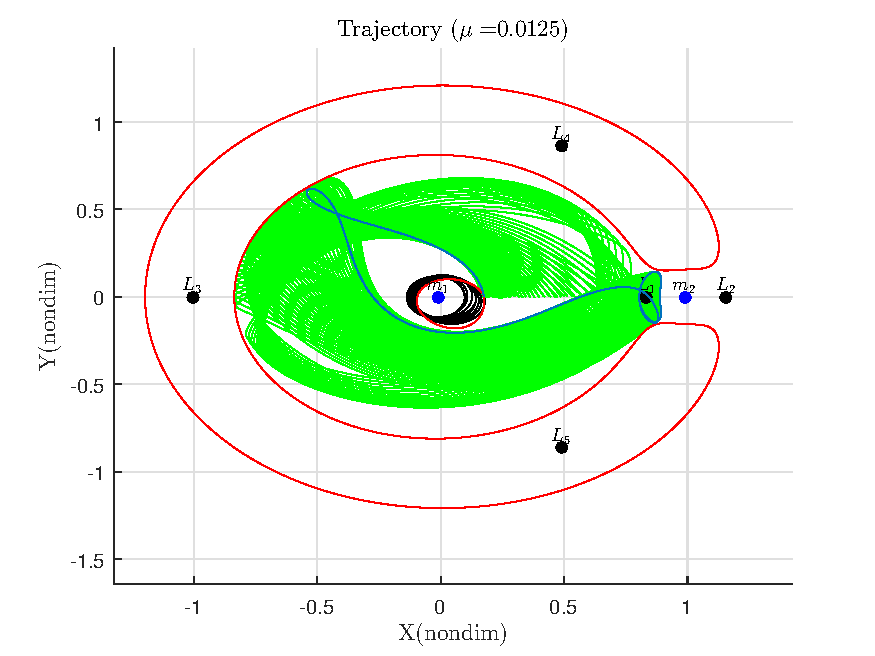
\includegraphics[width=\textwidth]{geo_transfer_full} }
               \only<2>{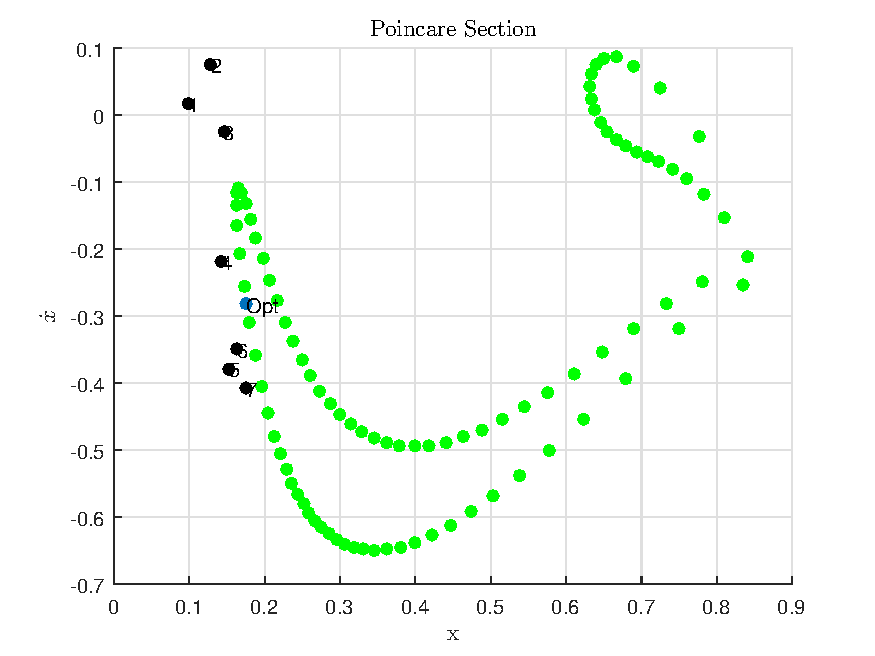
\includegraphics[width=\textwidth]{poincare}}
       \end{subfigure}
       \end{figure}

\end{frame} %--------------------------------------------%

\subsection{4769 Castalia}

\begin{frame}{Polyhedron Gravitation Model}

\begin{itemize}
    \item Potential is a function of only the shape model
    \item Globally valid, closed-form expression of potential
    \item Exact potential assumes a constant density 
    \item Accuracy solely dependent on shape model
\end{itemize}
\only<2>{
\begin{align*}\label{eq:potential}
    U(\vecbf{r}) &= \frac{1}{2} G \sigma \sum_{e \in \text{edges}} \vecbf{r}_e \cdot \vecbf{E}_e \cdot \vecbf{r}_e \cdot L_e - \frac{1}{2}G \sigma \sum_{f \in \text{faces}} \vecbf{r}_f \cdot \vecbf{F}_f \cdot \vecbf{r}_f \cdot \omega_f 
\end{align*}
}
\only<3>{
\begin{center}
  \animategraphics[autoplay,loop,width=0.5\textwidth]{30}{./animation/2016AAS/castalia/IMG}{00001}{00999}~\hfill
  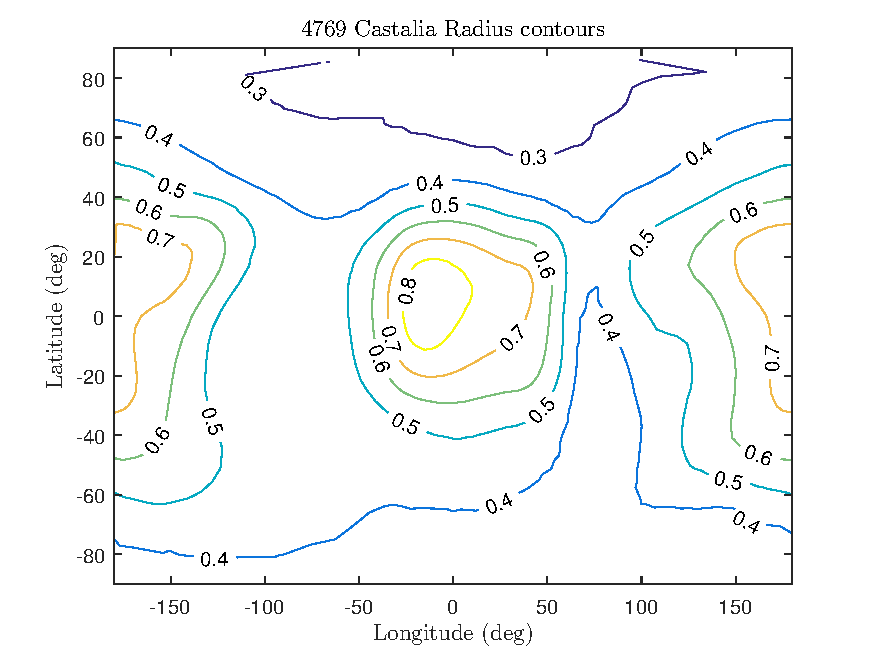
\includegraphics[width=0.5\textwidth]{figures/2016AAS/radius_contour.pdf}
\end{center}
}

\end{frame}

\begin{frame}{Simulation}

\begin{itemize}
    \item Generate the reachability set through discretization of \( \phi_i \)
    \item Visualize \( \Sigma \in \R^4 \) through the use of two 2-D sections
    \pause
    \item Control input allows for large deviation in velocity components
\end{itemize}

\begin{center}
    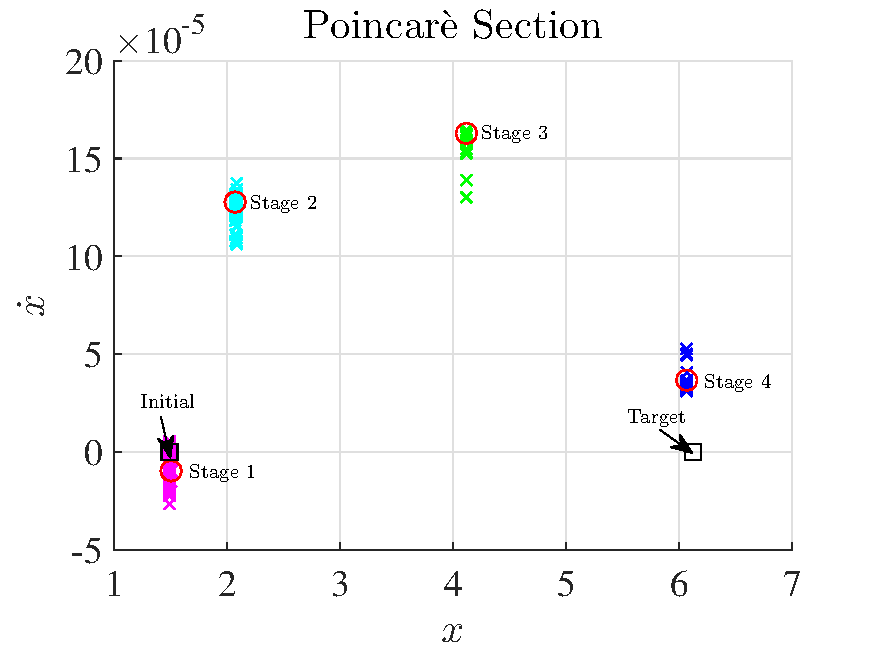
\includegraphics[width=0.5\textwidth]{figures/2016AAS/poincare_xvsxdot.pdf}
    \hfill
    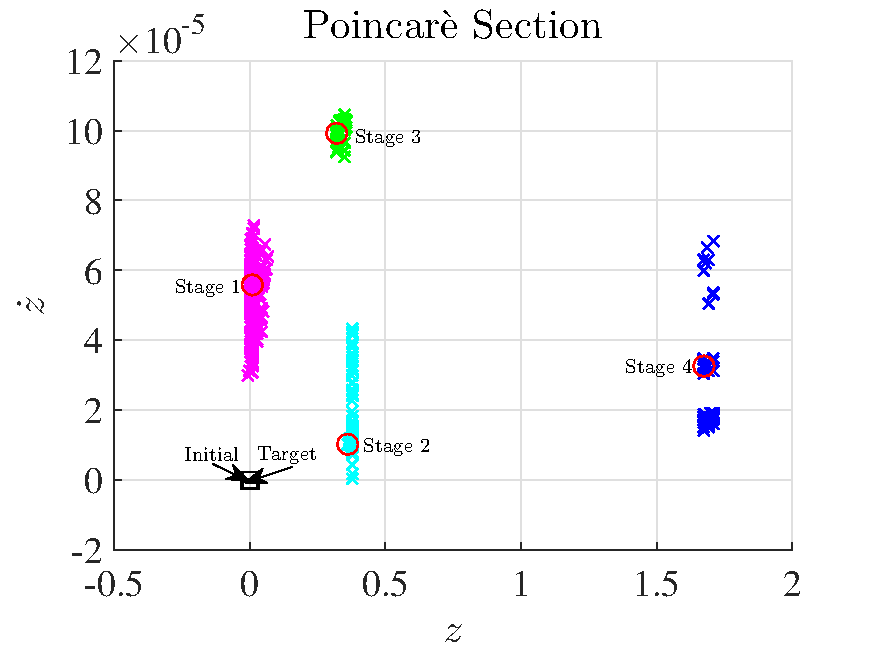
\includegraphics[width=0.5\textwidth]{figures/2016AAS/poincare_zvszdot.pdf}
\end{center}

\end{frame}

\begin{frame}{Simulation}
    \begin{itemize}
        \item Four iterations of the reachable state to meet the target set
        \item Final transfer is computed with a fixed terminal state constraint
    \end{itemize}

    \begin{center}
        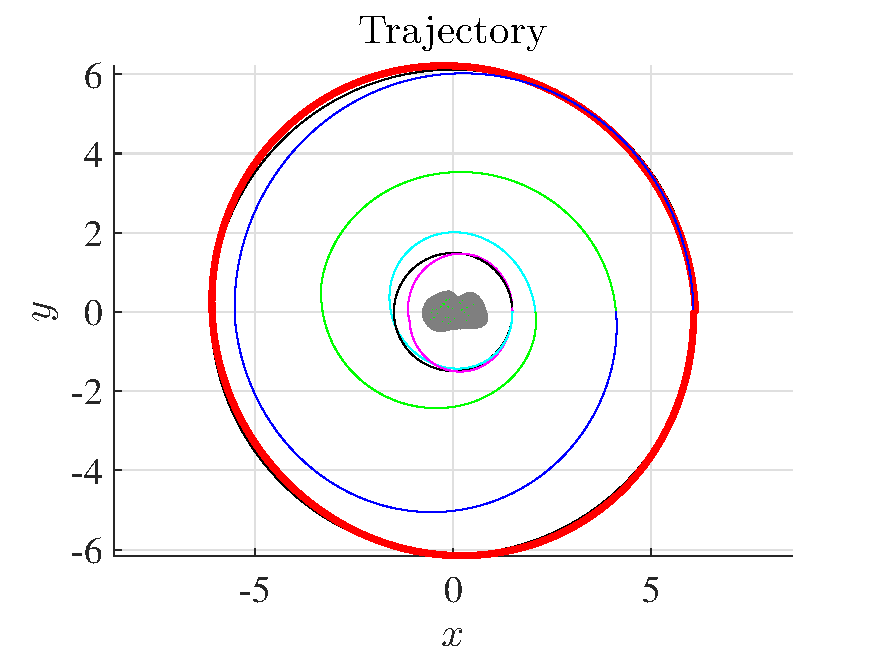
\includegraphics[width=0.5\textwidth]{figures/2016AAS/trajectory.pdf}
        \hfill
        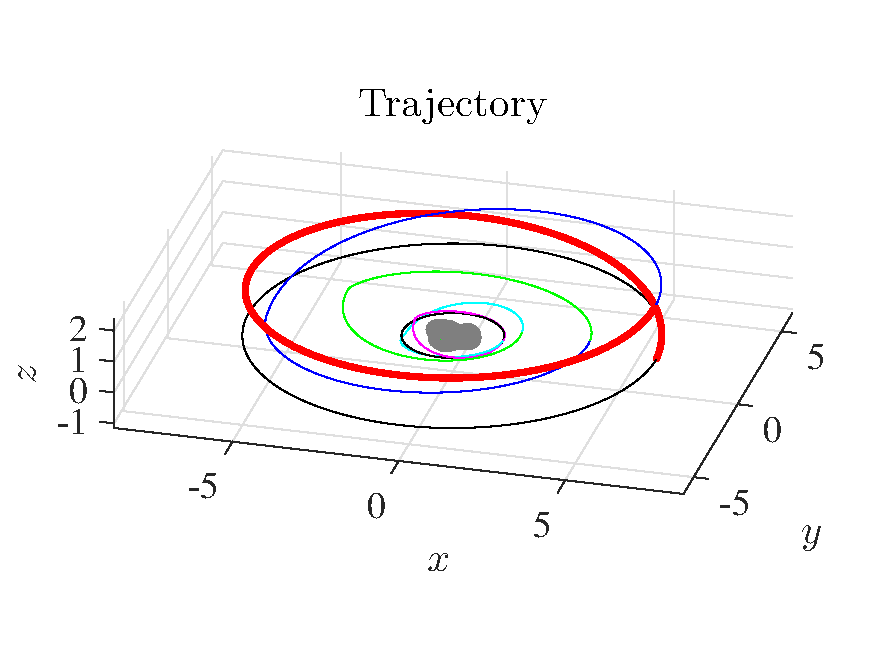
\includegraphics[width=0.5\textwidth]{figures/2016AAS/trajectory_3d.pdf}
    \end{center}

\end{frame}

\begin{frame}{Complete transfer}
\begin{itemize}
    \item We can visualize the complete trajectory in both the body and inertial frames
\end{itemize}

\begin{center}
  \animategraphics[autoplay,loop,width=0.5\textwidth]{30}{./animation/2016AAS/body/IMG}{00001}{01499}~\hfill
  \animategraphics[autoplay,loop,width=0.5\textwidth]{30}{./animation/2016AAS/inertial/IMG}{00001}{01499}
\end{center}

\end{frame}

\section{Constrained Attitude Control}
\subsection{Motivation}

\begin{frame} %--------------------------------%
	\frametitle{Motivation}
	\begin{itemize}
		\item Constrained rigid body attitude control
		\begin{itemize}
			\item Examples: spacecraft and robotic vehicles
			\item Attitude constraints: exposure concerns for optical payloads
			\begin{itemize}
				\item Bright objects: Sun, Moon
				\item Incoming debris
				\item Hostile action: directed energy
			\end{itemize}
		\end{itemize}
	\pause
	\item Previous approaches have several issues
	\begin{itemize}
		\item Attitude parameterizations: singularities/ambiguities
		\item Ad-hoc geometric approach: find intermediate points
		\item Randomized methods: stochastic stability result
		\item Barrier function: Motion planning/Optimal Control
	\end{itemize}
\end{itemize}
\end{frame} %----------------------------------%

\begin{frame}{Attitude Parameterizations}
	\begin{itemize}
		\item Euler Angles
		\begin{itemize}
			\item Minimal representation used for small attitude changes.
			\item Singularities exist for large angle slews: requires switching between 24 sequences
			\item Complicated trigonometric functions
		\end{itemize}
		\pause
		\item Quaternion 
		\begin{itemize}
			\item No singularities
			\item Two anti-podal quaternions for the same attitude
			\item Unwinding behavior 
		\end{itemize}
		\pause
		\item Geometric control
		\begin{itemize}
			\item Globally and uniquely characterize attitude: \( R \in \SO \)
			\item Singular representation of attitude 
			\item Geometrically exact
		\end{itemize}
	\end{itemize}
	
\end{frame}

\subsection{Research}

\begin{frame}{Research Objectives}
\begin{itemize}
	\item Attitude manuevers with state inequality constraints
	\item Barrier function approach on \( \SO \) 
	\begin{itemize}
		\item Aggressive, global manuevers free from singularities
	\end{itemize}
	\item Mathematically rigorous stability guarantee
\end{itemize}
\end{frame}

\begin{frame} %-----------------------------%
\frametitle{Attitude dynamics} 
\begin{itemize}

	\item Configuration space: rotation matrix from body frame to inertial frame
	 \[\SO =  \{R\in\R^{3\times 3}\,|\, R^TR=I,\;\mathrm{det}[R]=1\} \]
	\item Rigid body attitude dynamics:
\begin{gather*}
	J\dot\Omega + \Omega\times J\Omega = u+W(R,\Omega)\Delta \\
	\dot R = R\hat\Omega 
\end{gather*}
\end{itemize}

\end{frame}   %-----------------------------%

\begin{frame}{Constraints} %-------------------------------------------%
	\begin{itemize}
		\item Body fixed vector \( r \in \S^2\) - a light sensitive optical sensor
		\item Inertially fixed vector \( v \in \S^2 \) - bright object 
		\item Hard cone constraint:
		\[
			r^T R^T v \leq \cos \theta
		\]
	\end{itemize}
	\pause
	\begin{block}{Control Design Goal}
		Design control input \( u \) that stabilizes system from initial attitude \( R_0 \) to desired attitude \( R_d \) while satisfying constraint.
	\end{block}
\end{frame}%-------------------------------------%

\begin{frame}%-----------------------------------------------------%
\frametitle{Configuration Error Function}
\begin{itemize}
	\item Configuration error function used to quantify attitude error
        \[
        	\Psi(R) = A(R) B(R) 
        \]
	\item Combination of attractive and repulsive terms   
        \begin{gather*}
        	A(R) = \frac{1}{2} \tr{G \left( I - R_d^T R\right)} \\
        	B_i(R) = 1 - \frac{1}{\alpha_i} \ln \left( - \frac{ r^T R^T v_i - \cos \theta_i}{1 + \cos \theta_i}\right)
        \end{gather*}
\end{itemize}
\visible<2->{
\begin{figure} 
	\centering 	
	\begin{subfigure}[b]{0.3\textwidth} 
		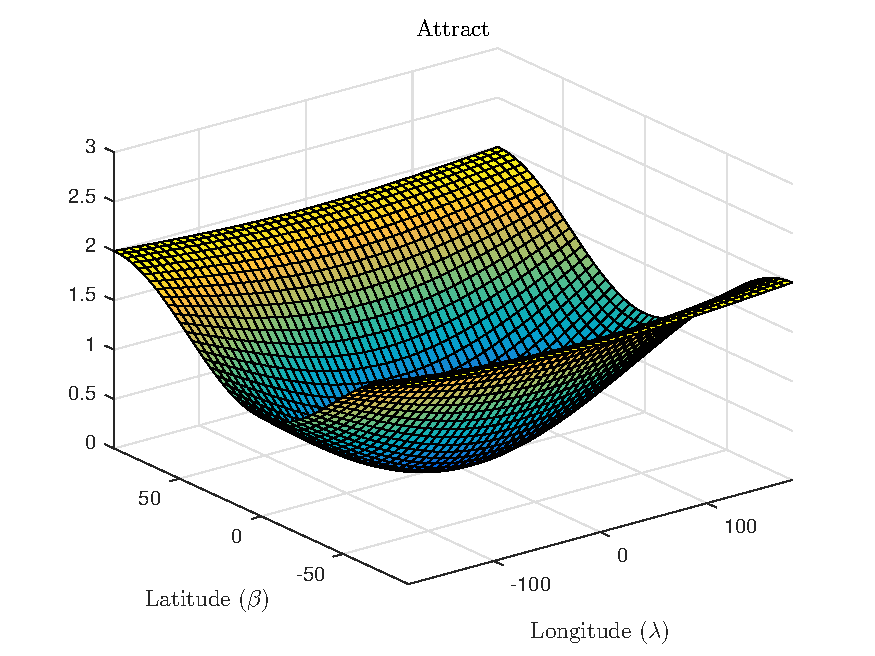
\includegraphics[width=\textwidth]{attract_error}
	\end{subfigure}~
	\begin{subfigure}[b]{0.3\textwidth} 
		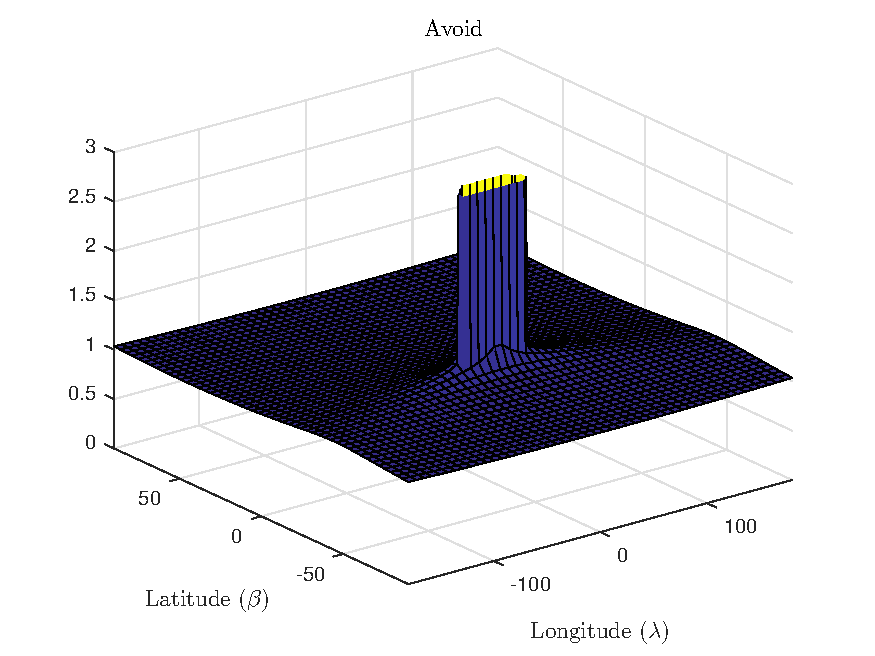
\includegraphics[width=\textwidth]{avoid_error}
	\end{subfigure}~
	\begin{subfigure}[b]{0.3\textwidth} 
		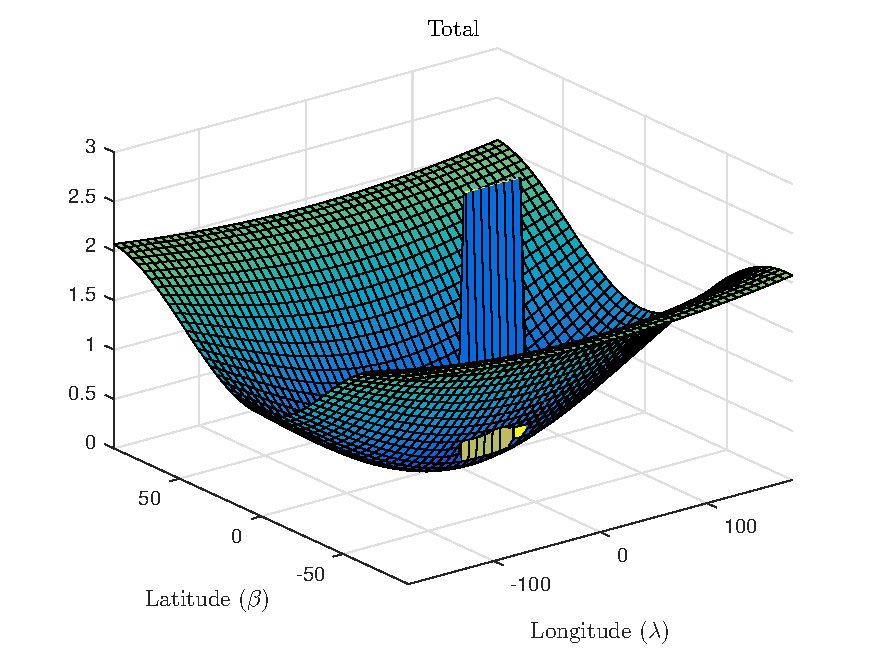
\includegraphics[width=\textwidth]{combined_error}
	\end{subfigure}
\end{figure}
}
\end{frame} %---------------------------------------------------%

\begin{frame}{Controller Design} %--------------------------------------------%
	\begin{block}{Adaptive Attitude Controller}
		Zero equilibrium of error vectors are Lyapunov stable, furthermore \( e_R , e_\Omega \to 0 \) as \( t \to \infty \)
		\begin{align*}
			u &= - k_R e_R - k_{\Omega} e_{\Omega} + \Omega \times J \Omega - W \bar{\Delta} \\
			\dot{\bar{\Delta}} &= k_\Delta W^T \parenth{ e_\Omega + c e_R }
		\end{align*}
	\end{block}
\end{frame}%--------------------------------------------------------------%

\subsection{Simulation results}

\begin{frame}{Simulation} %---------------------------------------------%
\begin{itemize}
	\item Can easily handle multiple constraints
	\item \href{https://youtu.be/dsmAbwQram4?t=20s}{UAV Experiment}
	\item Several benefits over previous methods:
		\begin{itemize}
			\item Avoids attitude parameterizations
			\item Efficient - feedback form
			\item Stability guarantee in spite of disturbances
		\end{itemize}
\end{itemize} 
\animategraphics[autoplay,loop,width=0.45\textwidth]{12}{./animation/sc_avoid_nodist/sc_avoid_nodist-}{0}{99}
\animategraphics[autoplay,loop,width=0.45\textwidth]{12}{./animation/sc_avoid_mult/sc_avoid_mult-}{0}{99}
\end{frame}%--------------------------------------------------%



\end{document}

